\begin{figure*}[t]
\begin{center}
\begin{small}
\begin{sc}
\begin{tabular}{r@{\hskip2pt}c@{\hskip2pt}c@{\hskip2pt}c@{\hskip2pt}c@{\hskip2pt}c@{\hskip2pt}c@{\hskip2pt}c@{\hskip2pt}c@{\hskip2pt}|@{\hskip2pt}M{\smallimg}}
a) & 1 & 2 & 3 & 4 & 5 & 6 & 7 & 8 & \\[3pt]
b) &\tabfigure{width=\smallimg}{fig/steps/1_masked.jpg} & \tabfigure{width=\smallimg}{fig/steps/2_masked.jpg} & \tabfigure{width=\smallimg}{fig/steps/3_masked.jpg} & \tabfigure{width=\smallimg}{fig/steps/4_masked.jpg} & \tabfigure{width=\smallimg}{fig/steps/5_masked.jpg} & \tabfigure{width=\smallimg}{fig/steps/6_masked.jpg} & \tabfigure{width=\smallimg}{fig/steps/7_masked.jpg} & \tabfigure{width=\smallimg}{fig/steps/8_masked.jpg} & Ground truth\\[13pt]
c) &\tabfigure{width=\smallimg}{fig/steps/1_out.jpg} & \tabfigure{width=\smallimg}{fig/steps/2_out.jpg} & \tabfigure{width=\smallimg}{fig/steps/3_out.jpg} & \tabfigure{width=\smallimg}{fig/steps/4_out.jpg} & \tabfigure{width=\smallimg}{fig/steps/5_out.jpg} & \tabfigure{width=\smallimg}{fig/steps/6_out.jpg} & \tabfigure{width=\smallimg}{fig/steps/7_out.jpg} & \tabfigure{width=\smallimg}{fig/steps/8_out.jpg}& {\raisebox{-.28\height}{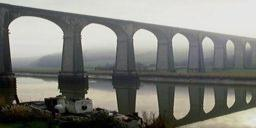
\includegraphics[width=\smallimg]{fig/steps/0_input.jpg}}}  \\[13pt]
d) &\tabfigure{width=\smallimg}{fig/steps/1_entropy.jpg} & \tabfigure{width=\smallimg}{fig/steps/2_entropy.jpg} & \tabfigure{width=\smallimg}{fig/steps/3_entropy.jpg} & \tabfigure{width=\smallimg}{fig/steps/4_entropy.jpg} & \tabfigure{width=\smallimg}{fig/steps/5_entropy.jpg} & \tabfigure{width=\smallimg}{fig/steps/6_entropy.jpg} & \tabfigure{width=\smallimg}{fig/steps/7_entropy.jpg} &&
\end{tabular}
\end{sc}
\end{small}
\end{center}
\vskip -0.1in
\caption{\textbf{Glimpse-based reconstruction step-by-step:} The figure shows a glimpse selection process based on AME for $8\times32^2$ glimpses for a sample $256\times128$ image. The rows correspond to \textsc{a)} step number, \textsc{b)} model input (glimpses), \textsc{c)} model prediction given, \textsc{d)} decoder attention entropy (known areas are explicitly set to zero). The algorithm explores the image in places where the reconstruction result is blurry.}
\label{fig:steps}
\end{figure*}